%-----------------------------------------------------------------------------------------------------------------------------------------------%
%	The MIT License (MIT)
%
%	Copyright (c) 2015 Jan Küster
%
%	Permission is hereby granted, free of charge, to any person obtaining a copy
%	of this software and associated documentation files (the "Software"), to deal
%	in the Software without restriction, including without limitation the rights
%	to use, copy, modify, merge, publish, distribute, sublicense, and/or sell
%	copies of the Software, and to permit persons to whom the Software is
%	furnished to do so, subject to the following conditions:
%	
%	THE SOFTWARE IS PROVIDED "AS IS", WITHOUT WARRANTY OF ANY KIND, EXPRESS OR
%	IMPLIED, INCLUDING BUT NOT LIMITED TO THE WARRANTIES OF MERCHANTABILITY,
%	FITNESS FOR A PARTICULAR PURPOSE AND NONINFRINGEMENT. IN NO EVENT SHALL THE
%	AUTHORS OR COPYRIGHT HOLDERS BE LIABLE FOR ANY CLAIM, DAMAGES OR OTHER
%	LIABILITY, WHETHER IN AN ACTION OF CONTRACT, TORT OR OTHERWISE, ARISING FROM,
%	OUT OF OR IN CONNECTION WITH THE SOFTWARE OR THE USE OR OTHER DEALINGS IN
%	THE SOFTWARE.
%	
%
%-----------------------------------------------------------------------------------------------------------------------------------------------%


%============================================================================%
%
%	DOCUMENT DEFINITION
%
%============================================================================%

%we use article class because we want to fully customize the page and dont use a cv template
\documentclass[10.5pt,A4]{article}	


%----------------------------------------------------------------------------------------
%	ENCODING
%----------------------------------------------------------------------------------------

%we use utf8 since we want to build from any machine
\usepackage[utf8]{inputenc}		

%----------------------------------------------------------------------------------------
%	LOGIC
%----------------------------------------------------------------------------------------

% provides \isempty test
\usepackage{xifthen}

%----------------------------------------------------------------------------------------
%	FONT
%----------------------------------------------------------------------------------------

% some tex-live fonts - choose your own

%\usepackage[defaultsans]{droidsans}
%\usepackage[default]{comfortaa}
%\usepackage{cmbright}
%\usepackage[default]{raleway}
%\usepackage{fetamont}
\usepackage{gillius}
%\usepackage[light,math]{iwona}
%\usepackage[thin]{roboto} 

% set font default
\renewcommand*\familydefault{\sfdefault} 	
\usepackage[T1]{fontenc}

% more font size definitions
\usepackage[10pt]{moresize}		

\usepackage{fontawesome}

%----------------------------------------------------------------------------------------
%	PAGE LAYOUT  DEFINITIONS
%----------------------------------------------------------------------------------------

%debug page outer frames
%\usepackage{showframe}			


%define page styles using geometry
\usepackage[a4paper]{geometry}		

% for example, change the margins to 2 inches all round
\geometry{top=0.6cm, bottom=-2cm, left=0.1cm, right=1cm} 	


%less space between header and content
\setlength{\headheight}{-5pt}		


%customize entries left, center and right
%\lhead{}
%\chead{ \small{Jan Küster  $\cdot$ Consultant and Software Engineer $\cdot$  Bremen, Germany  $\cdot$  \textcolor{sectcol}{\textbf{info@jankuester.com}}  $\cdot$ +49 176 313 *** **}}
%\rhead{}


%indentation is zero
\setlength{\parindent}{0mm}

%----------------------------------------------------------------------------------------
%	TABLE /ARRAY DEFINITIONS
%---------------------------------------------------------------------------------------- 

%for layouting tables
\usepackage{multicol}			
\usepackage{multirow}

%extended aligning of tabular cells
\usepackage{array}

\newcolumntype{x}[1]{%
>{\raggedleft\hspace{0pt}}p{#1}}%


%----------------------------------------------------------------------------------------
%	GRAPHICS DEFINITIONS
%---------------------------------------------------------------------------------------- 

%for header image
\usepackage{graphicx}

%for floating figures
\usepackage{wrapfig}
\usepackage{float}
%\floatstyle{boxed} 
%\restylefloat{figure}

%for drawing graphics		
\usepackage{tikz}				
\usetikzlibrary{shapes, backgrounds,mindmap, trees}


%----------------------------------------------------------------------------------------
%	Color DEFINITIONS
%---------------------------------------------------------------------------------------- 
\usepackage{transparent}
\usepackage{color}

%accent color
\definecolor{complcol}{RGB}{230,130,10}

%dark background color
\definecolor{bgcol}{RGB}{110,110,110}

%light background / accent color
%\definecolor{softcol}{RGB}{225,225,225}
\definecolor{softcol}{RGB}{95,95,95}

%\definecolor{sectcol}{RGB}{0,120,150}
\definecolor{sectcol}{RGB}{220,220,230}

%Package for links, must be the last package used
\usepackage[hidelinks]{hyperref}

%============================================================================%
%
%
%	DEFINITIONS
%
%
%============================================================================%

% returns minipage width minus two times \fboxsep
% to keep padding included in width calculations
\newcommand{\mpwidth}{\linewidth-\fboxsep-\fboxsep}
	

%----------------------------------------------------------------------------------------
% 	ARROW GRAPHICS in Tikz
%----------------------------------------------------------------------------------------

% a six pointed arrow poiting to the left
\newcommand{\tzlarrow}{(0,0) -- (0.2,0) -- (0.3,0.2) -- (0.2,0.4) -- (0,0.4) -- (0.1,0.2) -- cycle;}	

% include the left arrow into a tikz picture
% param1: fill color
%
\newcommand{\larrow}[1]
{\begin{tikzpicture}[scale=0.58]
	 \filldraw[fill=#1!100,draw=#1!100!black]  \tzlarrow
 \end{tikzpicture}
}

% a six pointed arrow poiting to the right
\newcommand{\tzrarrow}{ (0,0.2) -- (0.1,0) -- (0.3,0) -- (0.2,0.2) -- (0.3,0.4) -- (0.1,0.4) -- cycle;}

% include the right arrow into a tikz picture
% param1: fill color
%
\newcommand{\rarrow}
{
\begin{tikzpicture}[scale=0.7]
	\filldraw[fill=sectcol!100,draw=sectcol!100!black] \tzrarrow
 \end{tikzpicture}
}

%----------------------------------------------------------------------------------------
%	custom sections
%----------------------------------------------------------------------------------------

% create a coloured box with arrow and title as cv section headline
% param 1: section title
%
\newcommand{\cvsection}[1]
{
\colorbox{sectcol}{\mystrut \makebox[1\mpwidth][l]{
\larrow{bgcol} \hspace{-8pt} \larrow{bgcol} \hspace{-8pt} \larrow{bgcol} \textbf{\textcolor{black}{\uppercase{#1}}}\hspace{4pt}
}}\\
}

% create a coloured arrow with title as cv meta section section
% param 1: meta section title
%
\newenvironment{metasection}[1] {
	\vspace{0pt}
	\begin{center}
		\textcolor{black}{\large{\uppercase{#1}}}\\
	\normalsize
	\parbox{0.7\mpwidth}{\textcolor{black}	\hrule}
}{\end{center}}


%----------------------------------------------------------------------------------------
%	 CV EVENT
%----------------------------------------------------------------------------------------


% creates a stretched box as cv entry headline followed by two paragraphs about 
% the work you did
% param 1:	event time i.e. 2014 or 2011-2014 etc.
% param 2:	event name (what did you do?)
% param 3:	institution (where did you work / study)
% param 4:	what was your position
% param 5:	some words about your contributions
%
\newcommand{\volunteering}[3]{
\vspace{3pt}
	\begin{tabular*}{1\mpwidth}{p{1\mpwidth}  x{0.58\mpwidth}}
 	\textcolor{black}{\textbf{#1}} 

	\end{tabular*}
\vspace{-10pt}
\textcolor{softcol}{\hrule}
\vspace{6pt}
	\begin{tabular*}{0.5\mpwidth}{p{\mpwidth}}
\larrow{softcol}  \small #2\\[3pt]
\larrow{softcol}  \small #3\\[3pt]
	\end{tabular*}
}

\newcommand{\cveventzero}[3]{
\vspace{3pt}
	\begin{tabular*}{1\mpwidth}{p{0.4\mpwidth}  x{0.58\mpwidth}}
 	\textcolor{black}{\textbf{#2}} & \textcolor{complcol}{\small{#3}}, \textcolor{bgcol}{\small{#1}} 

	\end{tabular*}
\vspace{-10pt}
\textcolor{softcol}{\hrule}
\vspace{6pt}
}


\newcommand{\cveventone}[4]{
\vspace{3pt}
	\begin{tabular*}{1\mpwidth}{p{0.4\mpwidth}  x{0.58\mpwidth}}
 	\textcolor{black}{\textbf{#2}} & \textcolor{complcol}{\small{#3}}, \textcolor{bgcol}{\small{#1}} 

	\end{tabular*}
\vspace{-10pt}
\textcolor{softcol}{\hrule}
\vspace{6pt}
	\begin{tabular*}{0.5\mpwidth}{p{\mpwidth}}
\larrow{softcol}  \small #4\\[3pt]
	\end{tabular*}
}

\newcommand{\cveventtwo}[5]
{
\vspace{3pt}
	\begin{tabular*}{1\mpwidth}{p{0.4\mpwidth}  x{0.58\mpwidth}}
 	\textcolor{black}{\textbf{#2}} & \textcolor{complcol}{\small{#3}}, \textcolor{bgcol}{\small{#1}} 

	\end{tabular*}
\vspace{-10pt}
\textcolor{softcol}{\hrule}
\vspace{6pt}
	\begin{tabular*}{0.5\mpwidth}{p{\mpwidth}}
\larrow{softcol}  \small #4\\[3pt]
\larrow{softcol}  \small #5\\[3pt]
	\end{tabular*}

}

\newcommand{\cveventthree}[6]{
\vspace{3pt}
	\begin{tabular*}{1\mpwidth}{p{0.4\mpwidth}  x{0.58\mpwidth}}
 	\textcolor{black}{\textbf{#2}} & \textcolor{complcol}{\small{#3}}, \textcolor{bgcol}{\small{#1}} 

	\end{tabular*}
\vspace{-10pt}
\textcolor{softcol}{\hrule}
\vspace{6pt}
	\begin{tabular*}{0.5\mpwidth}{p{\mpwidth}}
\larrow{softcol}  \small #4\\[3pt]
\larrow{softcol}  \small #5\\[3pt]
\larrow{softcol}  \small #6\\[3pt]
	\end{tabular*}
}



% creates a stretched box as 
\newcommand{\cveventmeta}[2]
{
	\mbox{\mystrut \hspace{87pt}\textit{#1}}\\
	#2
}



%----------------------------------------------------------------------------------------
% CUSTOM STRUT FOR EMPTY BOXES
%----------------------------------------- -----------------------------------------------
\newcommand{\mystrut}{\rule[-.3\baselineskip]{0pt}{\baselineskip}}

%----------------------------------------------------------------------------------------
% CUSTOM LOREM IPSUM
%----------------------------------------------------------------------------------------
\newcommand{\lorem}
{Lorem ipsum dolor sit amet, consectetur adipiscing elit. Donec a diam lectus.}


% use to vertically center content
% credits to: http://tex.stackexchange.com/questions/7219/how-to-vertically-center-two-images-next-to-each-other
\newcommand{\vcenteredinclude}[1]{\begingroup
\setbox0=\hbox{\includegraphics{#1}}%
\parbox{\wd0}{\box0}\endgroup}

% use to vertically center content
% credits to: http://tex.stackexchange.com/questions/7219/how-to-vertically-center-two-images-next-to-each-other
\newcommand*{\vcenteredhbox}[1]{\begingroup
\setbox0=\hbox{#1}\parbox{\wd0}{\box0}\endgroup}

%----------------------------------------------------------------------------------------
%	ICON-SET EMBEDDING
%---------------------------------------------------------------------------------------- 

% at this point we simplify our icon-embedding by simply referring to a set of png images.
% if you find a good way of including svg without conflicting with other packages you can
% replace this part
\newcommand{\icon}[3]{\makebox(#2, #2){\textcolor{#3}{\raisebox{0pt}{\csname fa#1\endcsname}}}}	%icon shortcut
\newcommand{\icontext}[4]{ 						%icon with text shortcut
	\vcenteredhbox{\icon{#1}{#2}{#4}} \vcenteredhbox{\textcolor{#4}{#3}}
}
\newcommand{\iconhref}[5]{ 						%icon with website url
    \vcenteredhbox{\icon{#1}{#2}{#5}} \href{#4}{\textcolor{#5}{#3}}
}

\newcommand{\iconemail}[5]{ 						%icon with email link
    \vcenteredhbox{\icon{#1}{#2}{#5}} \href{mailto:#4}{\textcolor{#5}{#3}}
}



%============================================================================%
%
%
%
%	DOCUMENT CONTENT
%
%
%
%============================================================================%
\begin{document}
\fcolorbox{white}{white}{\begin{minipage}[c][0.95\textheight][t]{0.69\linewidth}


%---------------------------------------------------------------------------------------
%	TITLE HEADLINE
%----------------------------------------------------------------------------------------
\vspace{-3pt}
% use this for multiple words like working titles etc.
\hspace{-0.26\linewidth}
\colorbox{bgcol}{
	\makebox[1.5\linewidth][c]{
	\hspace{-5pt}\fontsize{29}{10}\selectfont{\textcolor{white}{\uppercase{Samuel Dubuis}}} 
	\textcolor{sectcol}{\rule[-1mm]{0.5mm}{0.9cm}}
	\parbox[b]{6cm}{\fontsize{17}{10}\selectfont{\textcolor{white}{{\uppercase{3 months summer job}}}}}%\\
% 	\large{ \textcolor{white}{{Project Assistant}}}}
}}

%% use this for single words, e.g. CV or RESUME etc.
%\colorbox{bgcol}{\makebox[\mpwidth][c]{\Huge{\textcolor{white}{\uppercase{Samuel Dubuis}} }\textcolor{sectcol}{\rule[-1mm]{0.5mm}{0.9cm}}\huge{ \textcolor{white}{\uppercase{6 months internship}}}}}

%----------------------------------------------------------------------------------------
%	HEADER IMAGE
%----------------------------------------------------------------------------------------


%\hspace{-1.6cm}
%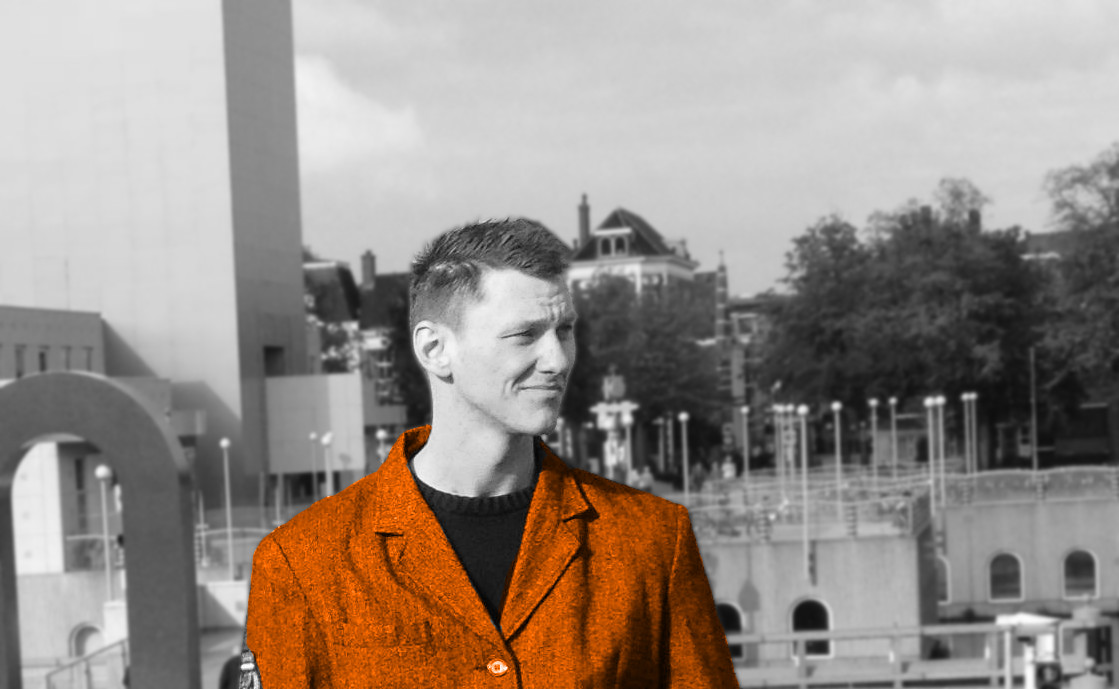
\includegraphics[trim= 0 250 0 270,clip,width=1\linewidth+3.1cm]{myfoto.jpg}	%trimming relative to image size!
%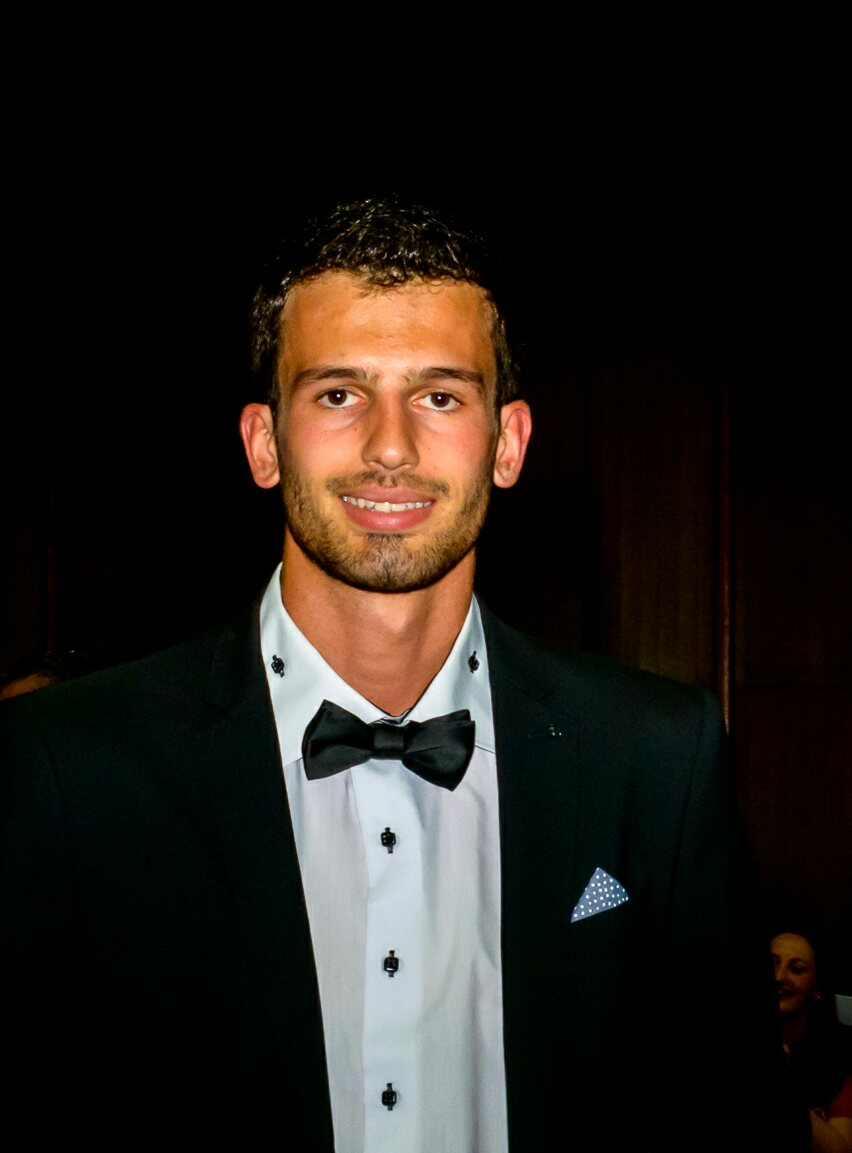
\includegraphics[trim= 350 150 0 200, clip ,width=\linewidth]{pp.jpg}	%trimming relative to image size

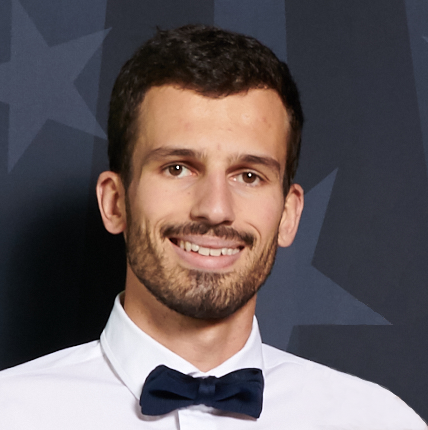
\includegraphics[scale=0.73]{pp_carre}

%---------------------------------------------------------------------------------------
%	SUMMARY
%----------------------------------------------------------------------------------------
\transparent{0.85}%
\vspace{-91pt}
\hspace{0.23\linewidth}
\colorbox{bgcol}{
	\parbox{0.745\linewidth}{
		\transparent{1}%
		\begin{center}
		\larrow{sectcol}\larrow{sectcol}\small\textcolor{white}{I recently gratuated from EPFL with a Bachelor in Communication Systems. I also am a basketball player in the second Swiss division, I’m very interested by sport, cinematography, any new technologies and anything that concerns computer science from close or far. Lastly studying in the Visual Computing field, and always ready to discover and learn ! I’m yet in the middle of my Master of Science in Communication Systems.}
		\end{center}
	}
}
\vspace{4pt}

%============================================================================%
%
%	CV SECTIONS AND EVENTS (MAIN CONTENT)
%
%============================================================================%

%---------------------------------------------------------------------------------------
%	STATUS
%----------------------------------------------------------------------------------------
%\cvsection{Status}
%
%JavaScript fullstack engineer, M.Sc. Digital Media, focuses on education and healthcare

%1\vspace{12pt}

%---------------------------------------------------------------------------------------
%	EXPERIENCE
%----------------------------------------------------------------------------------------
\cvsection{Experience}

%
\cveventthree{2018/06 - now}{Project Assistant / Auxiliary}{VPSI, EPFL}{Assistant/replacement of the operations manager which concerned the school’s websites production launch, the management of backups and sources of truth}{Creation and use of automation scripts, in Python, Bash and Ansible. Also worked on the development of WordPress plugins}{Support for the EPFL websites redesign project, which concerned the websites migration from Jahia to WordPress, implementation of the new graphical chart, support to webmasters and participation in the daily meetings}

\cveventone{2018}{Student Assistant}{CHILI Lab, EPFL}{TA during project sessions for the Introduction to Visual Computing course under Prof. Dillenbourg}

%\cveventone{2013-2018}{Fitter-Deliverer}{AJD Cuisines et Bains Sàrl, Sion, VS}{Summer job consisting of delivering and putting up kitchens and bathrooms, and after-%sale services}
%\textcolor{softcol}{\hrule}


\vspace{6pt}
%---------------------------------------------------------------------------------------
%	EDUCATION SECTION
%--------------------------------------------------------------------------------------
\cvsection{Formation}

\cveventone{2019/09 - now}{MSc. in Communication Systems}{École Polytechnique Fédérale de Lausanne}{Specialization in Signals, Images and Interfaces}

%\textcolor{softcol}{\hrule}

%
\cveventone{2015-2019}{BSc. in Communication Systems}{École Polytechnique Fédérale de Lausanne}{Visual Computing Track}

%
\cveventtwo{2011-2012}{Year Abroad}{Little Rock Catholic High School for Boys, USA}{A year of study and cultural experience in Arkansas, USA}{Consequently improved my english skills and had the opportunity to play basketball}

\vspace{6pt}



%---------------
%   PROJECTS
%---------------
\cvsection{Main Projects}

\begin{tabular*}{1\mpwidth}{p{0.7\mpwidth}x{0.28\mpwidth}}
\larrow{softcol} \small{BSc. Project : \textit{Simulation of moiré effects for counterfeit prevention}} & \textcolor{complcol}{\small{Innoview Sàrl \& IVRL Lab}}
\end{tabular*}

\begin{tabular*}{1\mpwidth}{p{0.59\mpwidth}x{0.39\mpwidth}}
\larrow{softcol} \small{Predicting photographers retouching with Deep Learning} & \textcolor{complcol}{\small{Computational Photo course EPFL}}
\end{tabular*}

\begin{tabular*}{1\mpwidth}{p{0.7\mpwidth}x{0.28\mpwidth}}
\larrow{softcol} \small{AICrowd.com project : \textit{Recommander system}} & \textcolor{complcol}{\small{ML course EPFL}}
\end{tabular*}

\begin{tabular*}{1\mpwidth}{p{0.7\mpwidth}x{0.28\mpwidth}}
\larrow{softcol} \small{Data over Sound : \textit{Exchange of files over the air using speakers}} & \textcolor{complcol}{\small{PDC course EPFL}}
\end{tabular*}

\begin{tabular*}{1\mpwidth}{p{0.7\mpwidth}x{0.28\mpwidth}}
\larrow{softcol} \small{Do you buy healthy ?: \textit{Big datasets analysis}}  & \textcolor{complcol}{\small{ADA course EPFL}}
\end{tabular*}

\begin{tabular*}{1\mpwidth}{p{0.7\mpwidth}x{0.28\mpwidth}}
\larrow{softcol} \small{See even more on my personnal page : samdubuis.github.io} & \textcolor{complcol}{\small{...}}
\end{tabular*}


\vspace{6pt}


%---------------
%    EXTRA PROFESIONNAL
%---------------
\cvsection{Extra-professional activities}

\volunteering{Volunteer for multiple events and organizations}{For SwissBasketball during Finals, National Team games and other basketball related events}{Barman for the club of Sion Basket and during the Lausanne 3x3 Masters}

\cveventone{2016-2020}{Basketball assistant coach}{AVsBa, ValBasket Camp}{Teaching of basketball in a pedagogical manner for younger ones, and in a more intensive manner for more experimented kids}

\cveventone{2010-2015}{Ski teacher}{Cours des Mayens}{Ski teaching for advanced young people during the Cours des Mayens}

\cveventzero{2014/2015 \& 2018/2020 season}{Team captain}{Sion Basket LNB}

\vspace{6pt}

%---------------
%    references
%---------------


\cvsection{References}

\begin{tabular*}{1\mpwidth}{p{1\mpwidth}x{0\mpwidth}}
\larrow{softcol} \small{\textbf{Emmanuelle Givord}, Chief Project Coordinator at EPFL, +41 79 158 75 20}
\end{tabular*} 

\begin{tabular*}{1\mpwidth}{p{1\mpwidth}x{0\mpwidth}}
\larrow{softcol} \small{\textbf{Professor Emeritus Roger Hersch}, Recommandation letter as supervisor}
\end{tabular*} 


\end{minipage}}%
\fcolorbox{white}{sectcol}{\begin{minipage}[c][0.95\textheight][t]{0.33\linewidth}

%----------------------------------------------------------------------------------------
%	META SECTION
%----------------------------------------------------------------------------------------
\vspace{6pt}
\begin{metasection}{Contact}

	\icontext{MapMarker}{12}{Lausanne, VD, Switzerland}{softcol}\\[4pt]
	\icontext{MobilePhone}{12}{+41 77 454 57 54}{softcol}\\[4pt]
	\iconemail{Send}{12}{samuel.dubuis@netplus.ch}{samuel.dubuis@netplus.ch}{softcol}\\[4pt]
	\iconhref{MousePointer}{12}{samdubuis.github.io}{http://samdubuis.github.io}{softcol}\\[4pt]
	\iconhref{Github}{12}{samdubuis}{https://github.com/samdubuis}{softcol}\\[4pt]
	%\iconhref{Twitter}{12}{@Kuester\_Jan}{https://twitter.com/kuester_jan?lang=en}{white}\\[6pt]
	\iconhref{Linkedin}{12}{/in/samueldubuis}{https://linkedin.com/in/samueldubuis}{softcol}\\[4pt]
	\icontext{Car}{12}{Driving Licence + CFF AG}{softcol}
	
\end{metasection}


\begin{metasection}{Languages}

\begin{tabular}{cc}
\textcolor{softcol}{French} & \raisebox{-2pt}{\icon{Star}{12}{complcol}\icon{Star}{12}{complcol}\icon{Star}{12}{complcol}\icon{Star}{12}{complcol}\icon{Star}{12}{complcol}} \\ 
\textcolor{softcol}{English - C1} & \raisebox{-2pt}{\icon{Star}{12}{complcol}\icon{Star}{12}{complcol}\icon{Star}{12}{complcol}\icon{Star}{12}{complcol}\icon{Star}{12}{complcol}} \\ 
\end{tabular}\\[2pt]
\textcolor{softcol}{\small\emph{( Certificate of Advanced English )}}
\begin{tabular}{cc}
\textcolor{softcol}{German - B1} & \raisebox{-2pt}{\icon{Star}{12}{complcol}\icon{Star}{12}{complcol}\icon{Star}{12}{white}\icon{Star}{12}{white}\icon{Star}{12}{white}} \\ 
\textcolor{softcol}{Italian - A2} & \raisebox{-2pt}{\icon{Star}{12}{complcol}\icon{Star}{12}{white}\icon{Star}{12}{white}\icon{Star}{12}{white}\icon{Star}{12}{white}} \\ 
\end{tabular} 

\end{metasection}
	

\begin{metasection}{Fields}

\icontext{Connectdevelop}{12}{Signals and Images Processing}{softcol}\\
\icon{Star}{12}{complcol}\icon{Star}{12}{complcol}\icon{Star}{12}{complcol}\icon{Star}{12}{complcol}\icon{Star}{12}{complcol}\icon{Star}{12}{complcol}\icon{Star}{12}{complcol}\icon{Star}{12}{complcol}\icon{Star}{12}{white}\icon{Star}{12}{white}\\[4pt]

\icontext{Code}{12}{Coding}{softcol}\\
\icon{Star}{12}{complcol}\icon{Star}{12}{complcol}\icon{Star}{12}{complcol}\icon{Star}{12}{complcol}\icon{Star}{12}{complcol}\icon{Star}{12}{complcol}\icon{Star}{12}{complcol}\icon{Star}{12}{complcol}\icon{Star}{12}{white}\icon{Star}{12}{white}\\[4pt]

\icontext{Server}{12}{Machine Learning}{softcol}\\
\icon{Star}{12}{complcol}\icon{Star}{12}{complcol}\icon{Star}{12}{complcol}\icon{Star}{12}{complcol}\icon{Star}{12}{complcol}\icon{Star}{12}{complcol}\icon{Star}{12}{complcol}\icon{Star}{12}{white}\icon{Star}{12}{white}\icon{Star}{12}{white}\\[4pt]

\icontext{Database}{12}{Data Analysis}{softcol}\\
\icon{Star}{12}{complcol}\icon{Star}{12}{complcol}\icon{Star}{12}{complcol}\icon{Star}{12}{complcol}\icon{Star}{12}{complcol}\icon{Star}{12}{complcol}\icon{Star}{12}{white}\icon{Star}{12}{white}\icon{Star}{12}{white}\icon{Star}{12}{white}\\[4pt]

\end{metasection}


\begin{metasection}{Technologies}

\textcolor{softcol}{
\icontext{Code}{12}{Python}{softcol} %\\[6pt]
\icontext{Code}{12}{MatLab}{softcol} %\\[6pt]
\icontext{Code}{12}{JAVA}{softcol} \\[6pt]
\icontext{Code}{12}{C/C++}{softcol} %\\[6pt]
\LaTeX \hspace{2pt} LaTeX%\\[6pt]
\icontext{Git}{12}{Git}{softcol} \\[6pt]
\icontext{Wordpress}{12}{WordPress}{softcol}
}
\end{metasection}

\begin{metasection}{Tools \& OS}

\textcolor{softcol}{
\icontext{Code}{12}{Jupyter}{softcol}
\icontext{Terminal}{12}{Terminal}{softcol}
\icontext{Cube}{12}{Blender}{softcol} \\[6pt]
\icontext{Image}{12}{GIMP}{softcol}
\icontext{Code}{12}{VS Code}{softcol} \\[4pt]
\textcolor{softcol}{\LARGE{\icon{Linux}{24}{softcol} \icon{Windows}{24}{softcol}}}
}
\end{metasection}

\begin{metasection}{Skills}
\\
\textcolor{softcol}{
Adapt easily $\cdot$ Sociable and spontaneous \\ Leadership $\cdot$ Teamwork $\cdot$ Responsible \\ Detail oriented $\cdot$ Motivated $\cdot$ Efficient}
\end{metasection}

\begin{metasection}{Activities}

\textcolor{softcol}{\LARGE{\icon{Dribbble}{24}{softcol} \icon{Headphones}{24}{softcol}  \icon{Tv}{24}{softcol}}}
\end{metasection}

%\begin{metasection}{Operating Systems}
%
%\textcolor{softcol}{\LARGE{\icon{Linux}{24}{softcol} \icon{Windows}{24}{softcol}}}
%
%\end{metasection}

%---------------------------------------------------------------------------------------
%	QR CODE (optional)
%----------------------------------------------------------------------------------------

\vspace{0pt}
\begin{center}

\includegraphics[width=0.30\mpwidth]{qr-code.png}
\end{center}

\end{minipage}}

%-------------------------------------------------------------------------------------------------
%	ARTIFICIAL FOOTER (fancy footer cannot exceed linewidth) 
%--------------------------------------------------------------------------------------------------

%\null
%\vspace*{\fill}
%\hspace{-0.25\linewidth}\colorbox{bgcol}{\makebox[1.5\linewidth][c]{\mystrut \small \textcolor{softcol}{Coypright 2018 jkuester@uni-bremen.de} $\cdot$ \textcolor{softcol}{licensed unter MIT license}}}

%============================================================================%
%
%
%
%	DOCUMENT END
%
%
%
%============================================================================%
\end{document}
